\documentclass[twoside,11pt]{article}

%================================ PREAMBLE ==================================

%--------- Packages -----------
\usepackage{fullpage}
\usepackage{amssymb}
\usepackage{amsmath}
\usepackage{amsthm}
\usepackage{latexsym}
\usepackage{graphicx}
\usepackage{wrapfig}
\usepackage{color}
\usepackage{url}
%\usepackage{algorithm,algorithmic}

%---------- Spacing ----------
\setlength{\parindent}{0pt}
\setlength{\parskip}{8pt}

%---------Definitions----------
\newcommand{\Yh}{\hat{\mathcal{Y}}}
\newcommand{\err}{\text{err}}
\newcommand{\regret}{\text{regret}}
\newcommand{\pred}{\text{\texttt pred}}

\newcommand{\half}{{\textstyle{\frac{1}{2}}}}
\renewcommand{\>}{{\rightarrow}}
\renewcommand{\hat}{\widehat}
\renewcommand{\tilde}{\widetilde}
\newcommand{\grad}{{\nabla}}
%
\newcommand{\argmax}{\textup{\textrm{argmax}}}
\newcommand{\argmin}{\textup{\textrm{argmin}}}
\newcommand{\argsort}{\textup{\textrm{argsort}}}
\newcommand{\sign}{\textup{\textrm{sign}}}
\newcommand{\poly}{\textup{\textrm{poly}}}
\newcommand{\er}{\textup{\textrm{er}}}
\newcommand{\zo}{\textup{\textrm{0-1}}}
\newcommand{\sq}{\textup{\textrm{sq}}}
%
\newcommand{\1}{{\mathbf 1}}
\newcommand{\0}{{\mathbf 0}}
\newcommand{\I}{{\mathbf I}}
\newcommand{\R}{{\mathbb R}}
\newcommand{\Z}{{\mathbb Z}}
\newcommand{\N}{{\mathbb N}}
\renewcommand{\P}{{\mathbf P}}
\newcommand{\E}{{\mathbf E}}
\newcommand{\Var}{{\mathbf{Var}}}
%
\renewcommand{\a}{{\mathbf a}}
\renewcommand{\b}{{\mathbf b}}
\renewcommand{\c}{{\mathbf c}}
\renewcommand{\d}{{\mathbf d}}
\newcommand{\f}{{\mathbf f}}
\renewcommand{\k}{{\mathbf k}}
\newcommand{\p}{{\mathbf p}}
\newcommand{\q}{{\mathbf q}}
\renewcommand{\u}{{\mathbf u}}
\newcommand{\w}{{\mathbf w}}
\newcommand{\x}{{\mathbf x}}
\newcommand{\y}{{\mathbf y}}
%
\newcommand{\A}{{\mathbf A}}
\newcommand{\bC}{{\mathbf C}}
\newcommand{\C}{{\mathcal C}}
\newcommand{\cD}{{\mathcal D}}
\newcommand{\F}{{\mathcal F}}
\renewcommand{\H}{{\mathcal H}}
\newcommand{\K}{{\mathbf K}}
\renewcommand{\L}{{\mathcal L}}
\newcommand{\bL}{{\mathbf L}}
\newcommand{\cN}{{\mathcal N}}
\newcommand{\W}{{\mathbf W}}
\newcommand{\X}{{\mathcal X}}
\newcommand{\bX}{{\mathbf X}}
\newcommand{\Y}{{\mathcal Y}}
%
\newcommand{\bloss}{{\boldsymbol \ell}}
\newcommand{\blambda}{{\boldsymbol \lambda}}
\newcommand{\bmu}{{\boldsymbol \mu}}
\newcommand{\bnu}{{\boldsymbol \nu}}
\newcommand{\bSigma}{{\boldsymbol \Sigma}}
\newcommand{\seta}{{\boldsymbol \eta}}
\newcommand{\bpsi}{{\boldsymbol \psi}}
\newcommand{\bphi}{{\boldsymbol \phi}}
\newcommand{\bPhi}{{\boldsymbol \Phi}}
\newcommand{\balpha}{{\boldsymbol \alpha}}
\newcommand{\bxi}{{\boldsymbol \xi}}

%=============================== END PREAMBLE ===============================

\begin{document}

%================================ COVER PAGE ================================

\emph{\footnotesize{CIS 620 Fall 2018, Project Report}}

\vspace{12pt}

\begin{center}

%Fill in your project title
\textbf{\Large{A Survey of Ranking Algorithms}}

\vspace{12pt}

%Fill in author names
Kishor Jothimurugan \\ (PennKey: \texttt{kishor}; Email: \texttt{kishor@seas.upenn.edu}) \\[4pt]
Nicolas Koh \\ (PennKey: \texttt{pennkey2}; Email: \texttt{email2@xxx.upenn.edu}) \\[4pt]
Mingyang Liu \\ (PennKey: \texttt{pennkey3}; Email: \texttt{email3@xxx.upenn.edu}) 

\end{center}

%---

%Add abstract 
\begin{abstract}
Abstract text goes here.
\end{abstract}

\vspace{12pt}

%============================= MAIN DOCUMENT ================================

\section{Introduction to Ranking}
In this project, we study the general problem of supervised ranking and survey
work in the area, paying attention to consistency results and
algorithms that perform empirically well but lack theoretical backing.

Roughly, the goal of supervised ranking is to learn from appropriate samples
in some way so as to learn how to rank, i.e., given a new set of $n$ items,
determine how they can be ordered so as to do well on some performance measure.

The canonical application is web search. Here, the search engine is given
a query $q$ and may find $n$ documents $v_1, \ldots, v_n$, but
has to determine an order in which they should be presented to a user.
Early on, this ordering was determined by hand-tuned models~\cite{bm25},
but there is good reason to believe that models adapting to collected data
(samples) would perform better. 

A sample is a (multi)set of instance-label pairs. Some appropriate types of samples are:
\begin{itemize}
\item (Binary relevance)
  $S = \{ ((q_i, (v_{i, j})_{j=1}^{n}), \y_i )\}_{i=1}^m$, where
  $\y_{i} \in \{0, 1\}^n$.
  That is, an instance is a query $q_i$ with a list of $n$ documents;
  the label for the instance is a vector $\y_i = (y_{i, j})_{j=1}^{n}$ indicating,
  for each document, whether it is relevant or not.
  This may be determined, e.g., by whether there is a
  user who clicked on the link or not.
\item (Relevance scores)
  $S = \{ ( (q_i, (v_{i, j})_{j=1}^{n}), \y_i )\}_{i=1}^m$,
  where $\y_i \in R^n \subseteq \R_+^n$.
  Same as the previous case, except that each document has a relevance
  score. 
  This may be determined, e.g., by the number of users who clicked on the link.
\item (Preference graphs) 
  $S = \{((q_i, (v_{i,j})_{j=1}^{n}), G_i)\})_{i=1}^m$, where $G_i$ is a weighted
  directed graph on the $n_i$ documents, all weights being non-negative.
  We can interpret $v_j \overset{w_{j,k}}{\to} v_k$ as saying that $v_j$ is
  preferred to $v_k$ with an importance weight of $w_{j,k}$.
  Note that this case subsumes the first two: a label for binary relevance
  can be coded as a directed bipartite graph in the obvious way
  with all weights $1$, and a label for relevance scores may be coded as a
  DAG with weights being the difference in scores.
  An important special case is when the graph consists
  of just a single edge, expressing a single pairwise preference.
  Preference graphs allow for cases where complete information on relevance is
  hard to obtain; for instance, an e-commerce ranking system may obtain $S$
  from a consumer survey, and surveyees should be allowed to specify
  preferences for only a small set of items. Ranking from preference graphs
  also have applications beyond just information retrieval, e.g., in
  recommendation systems and social choice theory, where we may want to
  aggregate preferences from different agents into a global ranking~\cite{}.
\end{itemize}
One may view relevance scores as a natural multiclass generalization of binary
relevance labels, and preference graphs as the
structured-prediction-generalization of relevance scores.

In each case, the goal is for the learning algorithm to learn from these samples
and output a ranking function
$f: Q \times D^n \to S_n$, where $Q$
is the set of queries, $D$ is the set of documents,
and $S_n$ is the set of permutations on $[n]$.
The formalism can be simplified by thinking of query-document pairs as feature
vectors in some space $\X$ (which is also done in practice), so
that dependence on queries can be dropped.

Formally, the supervised ranking problem can be framed as follows. There is an
instance space $\X$, a label space $\Y$ (which varies as above), and the
prediction space is $\Yh = S_n$. A permutation
$\sigma \in \Yh$ is interpreted such that $\sigma(i)$ is the position of the
$i$th item. A learning algorithm
takes $S = (\x_i, y_i)_{i=1}^m$ as input,
where $\x_{i} \in \X \subseteq \R^d$ is a feature vector
and $y_i \in \Y$ is a label following the cases above,
and outputs a function
$f_S: \X \to S_n$.
There is no loss of generality, since the feature space can in principle 
include $Q$ itself.

Performance of the learning algorithm is measured by some performance measure
$M: \Yh \times \Y \to \R_+$ or loss function
$\ell: \Yh \times \Y \to \R_+$. The goal is to minimize the $\ell$-risk
\begin{align*}
  \err_D^\ell[f_S] = \E_{({X}, Y) \sim D} [\ell(f_S({X}), Y)],
\end{align*}
for some unknown distribution $D$ on $\X \times \Y$ from which the samples
are drawn i.i.d.
The Bayes $\ell$-risk for a given distribution $D$ is the minimum possible
$\ell$-risk, denoted $\err^{l,*}_D = \inf_{f:\X \to \Yh} \err^l_D[f]$.
A learning algorithm is said to be $\ell$-consistent if for any distribution $D$,
\begin{align*}
  \err_D^l[f_S] \xrightarrow{\Pr} \err_D^{l,*}
  \quad \text{as} \quad
  m \to \infty,
\end{align*}
where $m = |S|$ is the sample size and the probability is over samples $S$ of
size $m$ which is drawn i.i.d. from $D$. Typically, minimizing the empirical
loss $\sum_{i=i}^m \ell(f(\x_i),y_i)$ over some suitable function class $\F_m$
gives a consistent algorithm but is computationally hard.
Therefore surrogate losses are used. Instead of learning a function from
$\X \to \Yh$, one typically learns a function $h_S:\X \to \C$ where the
surrogate space $\C$ is a convex set in $\R^d$ for some $d$. In the case of
ranking, $\C$ is usually $\R^n$ or $\R^{(n)(n-1)/2}$ which correspond to learning
pointwise and pairwise scores respectively.
The learned function is composed with a prediction map $\pred: \C \to \Yh$ to
map instances to permutations, $f_S = \pred \circ h_S$.

The function $h_S$ is obtained by minimizing a surrogate loss $\psi:\C \times \Y \to \R_+$ on the samples in $S$, $h_S \in \argmin_{h\in\H_m}\sum_{i=1}^m \psi(h(\x_i),y_i)$. This gives consistency w.r.t. $\psi$. Given a distribution $D$ over $\X \times \Y$, define $\psi$-risk as follows:
$$\err_D^\psi[h_S] = \E_{(X,Y)\sim D}[\psi(h_S(X),Y)]$$
The learning algorithm is $\psi$-consistent if $\err_D^\psi[h_S]$ converges in probablity to $\err_D^{\psi,*}$ as $m = |S|$ goes to infinity, where $\err_D^{\psi,*} = \inf_{h:\X \to \C}\err_D^\psi[h]$. A surrogate $\psi$ along with a prediction mapping $\pred$ is said to be $\ell$-consistent if $\psi$-consistency of a learning algorithm that outputs $h_S$ on input $S$ implies $\ell$-consistency of the algorithm that ouputs $f_S = \pred \circ h_S$ on input $S$.

Ramaswamy and Agarwal \cite{ramaswamy2016convex} showed that a property of
surrogates called $\ell$-calibration is sufficient for consistency of general
multiclass losses by extending the result for 0-1 loss in
\cite{tewari2007consistency}. They also define the notion of Convex Calibration
dimension which is the smallest $d$ for which there is a calibrated convex
surrogate with a surrogate space $\C \subseteq \R^d$. For most ranking
problems, this is bounded above by $n$ or $n^2$. 

There are many surrogates that are used in practice that are non-convex.
In such cases, one has to analyze the consistency and also the computational
complexity of emprical loss minimization. Some of the surrogates used in
practice are proven to be consistent whereas some are proven to be
inconsistent. There are a few practical approaches for which there are no
consistency results giving oppurtunity for further work in this area.
The surrogates for some the loss functions studied can be classified as
pointwise, pairwise and listwise. We do not categorize the surrogates
presented in this article. More information can be found in \cite{li2011short}.

% Some common measures and losses are:
% \begin{itemize}
% \item Precision: For binary relevance labels, 
%   \begin{align*}
%     \text{AvgPrec}@K(\sigma, (y_j)_{j=1}^n)
%     = \frac{1}{K} \sum_{r=1}^K \text{Prec}@r(\sigma, (y_j)_{j=1}^n)
%     = \frac{1}{K} \sum_{r=1}^K \frac{\sum_{j : \sigma(j) \leq r} y_j}{r}.
%   \end{align*}
%   Precision at $r$ is the proportion of relevant documents among those 
%   ranked up to $r$ according to $\sigma$. Average precision is the
%   non-truncated version of this measure, and mean average precision (MAP)
%   averages \text{AvgPrec} over all queries in a set, i.e.
%   \begin{align*}
%     \text{MAP}(\sigma, ((y_j)_{j=1}^{n_i})_{i=1}^m) =
%     \frac{1}{m} \sum_{i=1}^m \text{AvgPrec}(\sigma, (y_j)_{j=1}^{n_i}).
%   \end{align*}
% \item Normalized Discounted Cumulative Gain (NDCG): For relevance scores,
%   the discounted cumulative gain at $K$ is 
%   \begin{align*}
%     \text{DCG}@K(\sigma, (y_j)_{j=1}^n)
%     = \sum_{r=1}^K \frac{G(y_{\sigma^{-1}(r)})}{D(r)}
%     = \sum_{i: \sigma(i) \leq K} \frac{G(y_i)}{D(\sigma(i))}.
%   \end{align*}
%   (The first sum runs over positions and the second sum runs over
%   object indices.) The gain function $G$ boosts relevance scores, and is
%   normally taken to be $G(y) = 2^y - 1$. The discount function $D$ discounts
%   the importance of the term based on the position of the item, and is
%   normally taken to be $D(\sigma(i)) = \log(1 + \sigma(i))$. As before, DCG
%   is the non-truncated version of this, and NDCG normalizes DCG to obtain
%   a number in $[0,1]$, defined as
%   \begin{align*}
%     \text{NDCG}(\sigma, (y_j)_{j=1}^n)
%     = \frac{1}{N((y_j)_{j=1}^n)} DCG(\sigma, (y_j)_{j=1}^n),
%   \end{align*}
%   where
%   \begin{align*}
%     N((y_j)_{j=1}^n)
%     = \frac{1}{\max_{\sigma'} DCG(\sigma', (y_j)_{j=1}^n)} DCG(\sigma, (y_j)_{j=1}^n).
%   \end{align*}
%   In many applications, it is more important for the output to rank well for
%   items that are near the top compared to ones below, and to rank well for
%   highly relevant items compared to those with low scores; NDCG factors
%   these in using the discount and gain functions respectively.
% 
% \item Weighted pairwise disgreement loss: For preference graphs, the most
%   natural loss to define is just:
%   \begin{align*}
%     \ell_{\text{PD}}(\sigma, G)
%     = \sum_{j,k: j \neq k} w_{j,k}^G \1[\sigma(j) > \sigma(k)]
%   \end{align*}
%   Here the sum is over object indices, and we can take $w_{j,k}^G = 0$ if
%   the edge $j \to k$ is not in $G$. 
% \end{itemize}
% Note that while the pairwise disagreement (PD) loss is natural for preference
% graphs, and preference graphs generalize relevance scores, PD loss is not
% directly related to NDCG.
% 
% The ranking problem is difficult because the search
% space is exponentially large, and the ranking measures and losses are
% sensitive only to changes in rank and are hence flat or discontinuous
% everywhere (in the output of $h_S$). This makes it difficult to optimize
% using standard means like gradient descent. 
% 
% It is thus important to find good surrogate losses for these true losses, in
% particular ones that can be optimized efficiently for and are statistically
% consistent. For the rest of this report, we review consistency results and
% algorithms for NDCG and PD loss. 
% 
% A side note: since permutations are somewhat awkward, a common method is for
% the algorithm to output a scoring function  
% $h_S: \bigcup_{n=1}^\infty \X^n \to \mathbb{R}^n$ instead of a function returning
% permutations, and then sort with ties broken in some way. In the sequel,
% we switch presentation between scores $\vec{s}$ and permutations $\sigma$
% as appropriate, e.g., the measures above may be in terms of scores
% instead of $\sigma$.

% Beyond their distinct forms, the more salient point is that they exemplify
% different approaches to the problem.
% A pointwise loss is about determining the rank of an item directly.
% When training, a sample point $((x_{i,j})_{j=1}^{n_i}, y_i)$ may be broken up
% into sample points $\{(x_{i, j}, y_{i, j})\}_{j=1}^{n_i}$, and the loss may be
% minimized using techniques from ordinal regression~\cite{}.
% A pairwise loss is about determining when an item should be preferred to
% another. When training, a sample point $((x_{i,j})_{j=1}^{n_i}, y_i)$ may be
% broken up into sample points
% $\{ (x_{i, j_1}, x_{i, j_2}, y_{i, j_1}, y_{i, j_2}) \}_{j_1, j_2 \in [1, n_i]: j_1 \neq j_2}$.
% Suitable losses can be based on max-margin
% principles~\cite{ranking-with-large-margin-principle} or 
% some probability model of $\Pr[\text{$x_1$ is ranked higher than $x_2$}]$,
% e.g. KL-divergence~\cite{ranknet}. 
% A listwise loss is about determining the full ranking directly. Suitable losses
% may also be based on probabilistic models, but of
% $\Pr[\sigma \mid y = (y_{i,1} \ldots y_{i, n_i})]$ and/or
% $\Pr[\sigma \mid s = (s_{i,1} \ldots s_{i, n_i})]$~\cite{listmle, listnet}.
% Pairwise and listwise approaches outperform pointwise approaches~\cite{letor},
% intuitively because they exploit structure in the samples. For this reason, 
% we focus on pairwise and listwise approaches, and review consistency results
% and algorithms for binary relevance, NDCG and PD losses in the following
% sections.

The rest of the report is organized as follows.
In Section~\ref{sec:loss0-1} we look at the standard 0-1 loss on permutations.
In Section~\ref{sec:binary-relevance}, we consider surrogates for losses
defined for binary relevance labels.
In Section~\ref{sec:ndcg}, we consider surrogates for NDCG.
In Section~\ref{sec:pd}, we consider surrogates for PD loss.
In Section~\ref{sec:problems}, we look at extensions to ranking and other
problems considered in this project.

\section{0-1 Loss}\label{sec:loss0-1}
\section{Subset Ranking}\label{sec:binary-relevance}
Binary relevance, also known as subset ranking, is the case where the true labels are subsets of $[n]$, i.e., $\Y = \{0,1\}^n$. There are various loss functions in this setting most of which are low rank. Hence the quadratic surrogate loss for low rank losses defined in \cite{ramaswamy2013convex} can be applied directly to get consistent algorithms for these problems. Here, we look at a few important loss functions.

\subsection{Precision@$q$}
The precision@$q$ loss is a measure of how (im)precise the prediction is, with respect to the true label when we look at the prediction $\sigma$ as a map from $[n] \to \{0,1\}$ which sends the top $q$ positions to $1$ and the rest to $0$. More precisely, the loss $\ell_{P@q}: S_n \times \{0,1\}^n \to \R_+$ is defined by,
$$\ell_{P@q}(\sigma,\y) = 1 - \frac{1}{q}\sum_{i:\sigma(i)\leq q}y_i$$
A consistent surrogate loss $\psi_{P@q}:\R^n \times \{0,1\}^n \to \R_+$ and its corresponding prediction mapping $\pred_{P@q}:\R^n \to S_n$ are given by:
$$\psi_{P@q}(\u,\y) = \lVert \u - \y \rVert_2^2$$
$$\pred_{P@q}(\u) \in \argmax_{\sigma\in S_n}\sum_{i:\sigma(i)\leq q}u_i$$
In this case, the prediction mapping just amounts to sorting the indices in decreasing order of the $\u$ values. 

\subsection{MAP}
The mean average precision, as the name suggests, is a loss based on the avergae of precision at positions where the permutation maps the documents labelled 1 in $\y$. The loss $\ell_{\text{MAP}}:S_n \times \{0,1\}^n \to \R_+$ is given by,
$$\ell_{\text{MAP}}(\sigma,\y) = 1 - \frac{1}{\lVert\y\rVert_1}\sum_{i:y_i = 1}\frac{1}{\sigma(i)}\sum_{j:\sigma(j) \leq \sigma(i)}y_j$$
where $\lVert\y\rVert_1 = \sum_{i=1}^ny_i$ is the number relevant documents according to $\y$. It is known that there cannot be an $n$-dimensional convex calibrated surrogate for this loss. \cite{ramaswamy2013convex} gives an $O(n^2)$ dimensional surrogate for this loss. The consistent (convex) surrogate $\psi_{\text{MAP}}:  \R^{n(n+1)/2} \times \{0,1\}^n \to \R_+$ and the corresponding $\pred$ mapping is as follows:
$$\psi_{\text{MAP}}(\u,\y) = \sum_{i=1}^n\sum_{j=1}^i\Big(u_{ij} - \frac{y_iy_j}{\lVert\y\rVert_1}\Big)^2$$
$$\pred_{\text{MAP}}(\u) \in \argmax_{\sigma\in S_n}\sum_{i=1}^n\sum_{j=1}^i \frac{u_{ij}}{\max(\sigma(i),\sigma(j))}$$
This method involves learning a score for every unordered pair of documents/indices where a higher score indicates that both elements of the pair should be higher in rank. Unfortunately, there is no known polynomial time algorithm to compute the $\pred$ function. Therefore, one has to make low noise assumptions on the distribution $D$ to get fast algorithms. Under one such condition which assumes that the expected values of $y_{ii}/\lVert\y\rVert_1$ given any $x \in \X$ are more relevant than the cross terms $y_{ij}/\lVert\y\rVert_1$ where $i \neq j$, one can simply sort the indices in decreasing order of the diagonal terms $u_{ii}$ to compute the permutation from scores. In that scenario, it is also enough to just learn the diagonal terms giving an $n$-dimensional surrogate.  
\section{NDCG}
\label{sec:ndcg}
For relevance scores, the discounted cumulative gain at $K$ is 
\begin{align*}
  \text{DCG}@K(\sigma, (y_j)_{j=1}^n)
  = \sum_{r=1}^K \frac{G(y_{\sigma^{-1}(r)})}{D(r)}
  = \sum_{i: \sigma(i) \leq K} \frac{G(y_i)}{D(\sigma(i))}.
\end{align*}
(The first sum runs over positions and the second sum runs over
object indices.) The gain function $G$ boosts relevance scores, and is
normally taken to be $G(y) = 2^y - 1$. The discount function $D$ discounts
the importance of the term based on the position of the item, and is
normally taken to be $D(\sigma(i)) = \log(1 + \sigma(i))$. As before, DCG
is the non-truncated version of this, and NDCG normalizes DCG to obtain
a number in $[0,1]$, defined as
\begin{align*}
  \text{NDCG}(\sigma, (y_j)_{j=1}^n)
  = \frac{1}{N((y_j)_{j=1}^n)} DCG(\sigma, (y_j)_{j=1}^n),
\end{align*}
where
\begin{align*}
  N(y) = N((y_j)_{j=1}^n)
  = \frac{1}{\max_{\sigma'} \text{DCG}(\sigma', (y_j)_{j=1}^n)} \text{DCG}(\sigma, (y_j)_{j=1}^n)
\end{align*}
is the normalization factor. 
In many applications, it is more important for the output to rank well for
items that are near the top compared to ones below, and to rank well for
highly relevant items compared to those with low scores; NDCG factors
these in using the discount and gain functions respectively.

If the algorithm is to output a scoring function and has access to relevance
scores as labels, perhaps the simplest idea is to minimize similarity between
the function output and labels; when they are equal, the NCDG is also one.
In~\cite{bayes-optimal-subset-ranking}, it was
established that regression works: minimizing the least-squares
surrogate
\begin{align*}
  \phi(\vec{s}, y) = \sum_{j=1}^n {(s_j - y_j)}^2
\end{align*}
actually minimizes $1 - \text{NDCG}(\vec{s}, y)$ because we can upper bound
the latter by some multiple of the former. But this upper bound is coarse, and
the result does not imply consistency. 
Moreover, such a surrogate is pointwise, in the sense
that training is done on individual objects $(x_j, y_j)$, and does not
exploit potential structure in the problem.

In what is termed the pairwise approach, the surrogate loss
$\phi(\vec{s}, y)$ decomposes over pairs of objects rather than single objects
as above:
\begin{align*}
  \phi(\vec{s}, y)
  &\stackrel{\Delta}{=}
  \sum_{j,k : i \neq j} \phi'(s_j - s_k, y_j - y_k) \\
  \phi(\vec{s}, G)
\end{align*}
for some $\phi'$. The pairwise approach attempts to reduce the problem of
ranking to the problem of determining when an object should be preferred over
another. Some choices of surrogate include the hinge loss, 

So a starting point is to define
a probabilistic model for $\Pr[x_j \to x_k]$, i.e.\ the probability that $x_j$
should be ranked higher than $x_k$. RankNet~\ref{ranknet} is a major
representative 

In the listwise approach, the structure of the entire 

Empirical comparisons also show that pointwise
surrogates like these, where training is done on individual objects, are less
accurate than pairwise and listwise surrogates; a pairwise surrogate is of the
form
\begin{align*}
  \phi(\vec{s}, y)
  &\stackrel{\Delta}{=}
  \sum_{j,k : i \neq j} \phi'(s_j - s_k, y_j - y_k) \\
  \phi(\vec{s}, G)
  &\stackrel{\Delta}{=}
  \sum_{j,k : i \neq j} \phi'(s_j - s_k, w_{j,k}^G) 
\end{align*}
for some $\phi'$, i.e., the loss decomposes over pairs.

Moreover, this surrogate is a pointwise surrogate;
when training on this loss, 



Subsequent work showed that
direct regression works~\cite{ndcg-consistency}: 

The idea of making function output and labels similar
also lies behind using cosine similarity~\cite{rank-cosine}, 
However, 


\subsection{LambdaRank}

\section{Pairwise Disagreement Loss}\label{sec:pdloss}


In terms of consistency, Duchi et.\ al.~\cite{duchi2010ranking}
studied the consistency of pairwise
surrogates, and proved that a surrogate is consistent w.r.t. a
loss $\ell(\sigma, G)$ that is sensitive only to changes in rank
(e.g.\ PD loss and NDCG) iff it is $\ell$-calibrated (called edge-consistent
in that paper). Using calibration, they showed that Ranking SVM and RankBoost
are inconsistent w.r.t.\ PD loss, even under a low-noise assumption.
However, empirical success of these pairwise surrogates led to another study
that generalized edge-consistency/calibration to a condition they called
rank-consistency.
Roughly, a surrogate is rank-consistent if all its minimizers
disagree with every non-minimizer of $\ell$ on some pair. Under a condition
on distributions that they call rank-differentiability,
similar to the low-noise condition, weighted pairwise surrogates are consistent
w.r.t.\ PD loss. The surrogates of Ranking SVM, RankBoost, and RankNet, are
all instances, and are hence consistent w.r.t.\ PD loss.


\cite{duchi2010ranking} studies consistency of pdloss. They show two widely used surrogates are not generally consistent. Then they gives low.noise condition on the probability distribution under which we can have calibrated surrogate loss. \cite{ramaswamy2013convex} generalizes low.noise condition and provides another more general condition and surrogate loss. 

Unfinished

\section{Variations of Ranking and Other Problems}\label{sec:problems}
In this section, we give an overview of some problems we considered in the
course of the project, motivated by papers we were reading~\cite{}. 

One direction was along ranking. In the ranking problem, the prediction space
is the set of permutations, which one can think of as the set of total orders.
We considered generalizing this to partial orders with possibly some
restriction, and identified task scheduling as an application domain.
We outline how ranking algorithms may be applied to solve some
problems in these domains.

Another direction was along online expert advice.
TODO.

These are discussed in the sections below.


\subsection{Task scheduling}
Consider a cloud service that offers distributed infrastructure to process
jobs, or a modern data processing system that processes queries on large
databases.
In such systems, queries may be passed to an execution planner
which uses statistics, current workloads, and cost models to choose an optimal
plan among a set of candidate execution plans.
These plans are in the form of directed acyclic graphs with edges indicating
task dependencies.
Some metrics for choosing plans include makespan (time to finish executing
the DAG) and resource consumption (e.g., to obtain fairness between queries).
One challenge, however, is that available resources change with time,
so an execution plan deemed optimal before execution can become sub-optimal
during its lifetime~\cite{mahajan2018qoop}.

With this as setting, one may consider learning a decision rule for
scheduling tasks.
We consider $\X$ to be some set of feature vectors
(extracted from the query, tasks, resources at time of execution,
time-of-day, and so on), and $\Y$ to be the set of preference graphs with
appropriate augmentation depending on the metric of interest. Samples
$S = \{((x_{i,j})_{j=1}^{n_i}, y_i)_{i=1}^m\}$ may come from computing the best DAG
in hindsight and collecting statistics. We want the learning algorithm to
output a DAG that minimizes $\ell$-risk for some suitable loss $\ell$.

If we make the simplification that execution of plans proceed in rounds (e.g.\
MapReduce), ranking techniques can be brought to bear. Specifically,
let the prediction space be
$\Yh = \{f: \bigcup_{i=1}^n \X^n \to \mathbb{Z}_+\}$,
i.e.\ functions which stratifies jobs into rounds. This is no different from
functions that output relevance scores.

\subsubsection{Minimizing Job Completion Time and Parallel Processing Cost?}
Here, we want the scoring function to output as few rounds as possible.
A way to do this is as follows. For $r$ items, let
\begin{align*}
  \Y_r &= \{ (G, \vec{c})
  \mid \text{$G$ is a weighted DAG on $[r]$ and $\vec{c} =( c_1, \ldots, c_r), c_1< ...< c_r$}
  \}.
\end{align*}
The label space is $\Y = \Y_r$ is a set of finite number of weighted DAGs
over $r$ items. We interpret each $c_i$
to be the unit cost incurred for scheduling a task past round $i$.
The prediction space $\mathcal{T}$ has size $r^r$

The loss $\ell$ can then be defined as:
\begin{align*}
  \ell(f, (G, \vec{c}))
  = \sum_{i,j: i \neq j} w_{i,j}^G \1_{f(i) \geq f(j)}
  + \sum_{i=1}^n c_i \sum_{j=1}^n \1_{f(j) \geq i}
\end{align*}


\textcolor{red}{Mingyang: The loss defined below eq(1) is easier to analyze and have the same property to penalize depth.}


%%%%%%%%%%%%%%%%%%%%%%%%%%%%%%%
\subsubsection{Mingyang's draft for Minimizing Job Completion Time}

TODO:
\begin{itemize}
\item Nicolas: Explanation of the problem, possibility of using ranking
  algorithms to solve this problem. 
\item Shivani's method that justifies using squared loss as a surrogate
  (justification: it is consistent). This reduces the problem to just a
  clustering problem giving a ranking.
\item Connection between surrogate score output $u_{ij}$'s and the analysis
  of the expected graph. Clarifying notation that $y_{ij} = \E_G[y_{ij}]$.
\item Preliminary result: Under some assumptions on the distribution of graphs,
  the Bayes-consistent clustering must respect the Bayes-consistent ranking.
\item Change $m$ to $\sigma^*$ in Assumption.
\item Strengthen clusters to adjacent clusters in proof. 
\item Using uniqueness condition in proof. 
\end{itemize}

\iffalse
Let consider $5$ items. The true permutation $\sigma^*: \sigma^*(i)=i$. If we have a mapping $m$ with $m(1)=1, m(2,4)=2, m(3,5)=3$, then it has a wrong ranking for pair $(3,4)$. Let $m'$ be the flip mapping. 
\begin{itemize}
	\item $l(m)=y_{24}+y_{42}+y_{35}+y_{53}+y_{34}$
	\item $l(m')=y_{23}+y_{32}+y_{45}+y_{54}$
\end{itemize}
If $y_{34}=1, y_{43}=0$, which is the only edge in the difference, and $y_{24}=y_{42}=0,y_{35}=y_{53}=0$, $y_{23}=y_{32}=1, y_{45}=y_{54}=0$. Then $l(m)=1<l(m')=2$
\fi


\begin{equation}\label{eq:pdloss}
\begin{split}
%\text{Target Loss: }l: \mathcal{Y}\times\mathcal{T}, \text{ with } l((\mathbf{y},\mathbf{c}),  m)=\sum\limits_{i\not=j}y_{ij}1_{\{m(i)\geq m(j)\}}+\sum\limits_{i=1}^rc_i\big(\sum_{j=1}^r1_{\{m(j)\geq i\}}\big)=(\mathbf{y}', \mathbf{c}')\begin{pmatrix} \mathbf{\Phi}_1(m) \\\mathbf{\Phi}_2(m) \\\end{pmatrix} 
\text{Target Loss: }l: \mathcal{Y}\times\mathcal{T}, \text{ with } l((\mathbf{y},\mathbf{c}),  m)=\sum\limits_{i\not=j}y_{ij}1_{\{m(i)\geq m(j)\}}+\sum\limits_{i=1}^rc_i1_{\{(\max_jm(j))\geq i\}}=(\mathbf{y}', \mathbf{c}')\begin{pmatrix} \mathbf{\Phi}_1(m) \\\mathbf{\Phi}_2(m) \\\end{pmatrix} 
\end{split}
\end{equation}
, where $\mathbf{\Phi}_1(m)$ is $r(r-1)$ length vector with entries $1_{\{m(i)\geq m(j)\}}$, and  $\mathbf{\Phi}_2(m)$ is $r$ length vector with entries $1_{\{(\max_jm(j))\geq i\}}$.  By Theorem 3 \cite{ramaswamy2013convex}, we have $l$-calibrated surrogate $(\psi_l^*, \text{pred}_l^*)$ , where
\begin{equation*}
\begin{split}
\psi_l^*((\mathbf{y},\mathbf{c}), (\mathbf{u}, \mathbf{v}))=\sum\limits_{i\not=j}^{r}(u_{ij}-y_{ij})^2+\sum\limits_{k=1}^r(v_k-c_i)^2,\quad \text{pred}_l^*(\mathbf{u}, \mathbf{v})\in\text{argmin}_{m\in \mathcal{T}}\bigg(\mathbf{u}'\mathbf{\Phi}_1(m)+\mathbf{v}'\mathbf{\Phi}_2(m)\bigg)
\end{split}
\end{equation*}
It is easy to see that solving $\text{pred}_l^*$ is same as solving original PD-loss problem. 



Let $m^*: [r]\rightarrow [r]$ be the optimal solution of eq(\ref{eq:pdloss}), and let $|m|=\max_jm(j)$. We notice that $m$ must satisfies the below two rules.
\begin{lemma}
	Fact1(no gap): For any $k\in[|m|]$, $m^{-1}(k)\not=\emptyset$. 
\end{lemma}
\begin{proof}
If there exists such a $k$, then we can move all the items ranked lower than $k$ w.r.t $m$ by one level, i.e, set $m'(l)=m(l)-1, \forall l, m(l)>k$. We can reduce the target loss by $c_{|m|}>0$, which contradicts that $m$ is optimal.
\end{proof}

Before deriving the second fact, we first re-examine the target loss. The target loss can be written as three parts: pdloss, clusterloss, depthloss$$\sum\limits_{i\not=j}y_{ij}1_{\{m(i)> m(j)\}}+\sum\limits_{i\not=j}y_{ij}1_{\{m(i)= m(j)\}}+\sum\limits_{i=1}^rc_i1_{\{(\max_jm(j))\geq i\}}$$

\begin{assumption}
	There is a unique total order $\sigma^*$. For any  $i\not=j $, wlog $m(i)<m(j)$
	$$y_{ij}+y_{ji}\geq \sum\limits_{k\in \{l: \sigma^*(l)\in [m(i), m(j)]\}, l={(\sigma^*)}^{-1}(\sigma^*(k)+1)\}}y_{kl}+y_{lk}$$
\end{assumption}
It means under total ranking, clustering two nodes will incur strict bigger loss than sum of  clustering loss of any two items between them. 

\begin{lemma}
Fact2(respect DAG): If $\sigma^*(k)<\sigma^*(l)$, then $m(k)\leq m(l)$.
\end{lemma}
\begin{proof}
	If not, then for $m$, there must exist two clusters which do not respect DAG. That is to say, for some $k<l$, and let the first cluster $C_1=\{i: m(i)=k\}$, the second $C_2=\{j:m(j)=l\}$, $\exists \text{ pair } (i,j)\in (C_1, C_2)$, $\sigma^*(i)>\sigma^*(j)$. Now consider $m'$ which flip all these pairs of $m$ until we can not find more such pairs. and keep the rest of clusters unchanged. When we cannot find more such pairs, let $C_{1,u}$ be items previously in $C_1$ and now still in $C_1$;   $C_{1, d}$ be items previously in $C_1$ but now in $C_2$;  et $C_{2,u}$ be items previously in $C_2$ but now in $C_1$;   $C_{2, d}$ be items previously in $C_2$ and now still in $C_2$. Since we only do flip pairs, $|C_{1,d}|=|C_{2,u}|$.
	\begin{equation}
	\begin{split}
	&C_1=  C_{1,u}\cup C_{1,d}\\
		&C_2=  C_{2,u}\cup C_{2,d}\\
		&m: m(C_1)=k; m(C_2)=l\\
		&m': m'(C_{1, u}\cup C_{2, u})=k; m'(C_{1,d}\cup C_{2, d})=l\\
	\end{split}
	\end{equation}
	\begin{itemize}
		\item pdloss: $m'$ will have no greater pdloss than $m$, because $m'$ respect more ranking than $m$.
		\item depthloss: $m$ and $m'$ have same depthloss.
		\item clusteringloss: let $C_{cl}(m)$, $C_{cl}(m')$ be clusteringloss for $m, m'$
		\begin{itemize}
			\item $C_{cl}(m)=\bigg(\sum\limits_{i\in C_{1, u}, j\in C_{1, u}}y_{ij} + \sum\limits_{i\in C_{2, d}, j\in C_{2, d}}y_{ij} \bigg)+ \bigg(\sum\limits_{i\in C_{1, u}, j\in C_{1, d}}(y_{ij}+y_{ji}) \bigg)+\bigg( \sum\limits_{i\in C_{2, u}, j\in C_{2, d}}(y_{ij}+y_{ij})\bigg)$
						\item $C_{cl}(m')=\bigg(\sum\limits_{i\in C_{1, u}, j\in C_{1, u}}y_{ij} + \sum\limits_{i\in C_{2, d}, j\in C_{2, d}}y_{ij} \bigg)+ \bigg(\sum\limits_{i\in C_{1, u}, j\in C_{2, u}}(y_{ij}+ y_{ij})\bigg)+\bigg( \sum\limits_{i\in C_{1, d}, j\in C_{2, d}}(y_{ij}+y_{ij})\bigg)$
		\end{itemize}
	By our flip rule, $\sigma^*(i)>\sigma^*(j)$ for any $i\in C_{1,d}\cup C_{2,d}, j\in C_{2,u}\cup C_{1,u}$. If not, the fliping process will not stop. Since the first big bracket is same for $m$ and $m'$, we only work on the rest two. For any $i\in C_{1,u}$, $j\in C_{2,d}, k\in C_{2,u}, l\in C_{1,d} $, There are four possibilities:
	\begin{itemize}
		\item $\sigma^*(k)<\sigma^*(i)<\sigma^*(j)<\sigma^*(l)$
			\item $\sigma^*(k)<\sigma^*(i)<\sigma^*(l)<\sigma^*(j)$
				\item $\sigma^*(i)<\sigma^*(k)<\sigma^*(j)<\sigma^*(l)$
					\item $\sigma^*(i)<\sigma^*(k)<\sigma^*(l)<\sigma^*(j)$
	\end{itemize}
For the first case
\begin{equation*}
\begin{split}
(y_{il}+y_{li})+(y_{kj}+y_{jk})&\geq (y_{ij}+y_{ji}+y_{jl}+y_{li}) + (y_{ki}+y_{ik}+y_{ij}+y_{ji})\\
&>y_{ik}+y_{ki}+y_{jl}+y_{lj}\\
\end{split}
\end{equation*}
For the second case
\begin{equation*}
\begin{split}
(y_{il}+y_{li})+(y_{kj}+y_{jk})&\geq (y_{il}+y_{li}) + (y_{ki}+y_{ik}+y_{ij}+y_{ji}+y_{lj}+y_{jl})\\
&>y_{ik}+y_{ki}+y_{jl}+y_{lj}\\
\end{split}
\end{equation*}
For the third case
\begin{equation*}
\begin{split}
(y_{il}+y_{li})+(y_{kj}+y_{jk})&\geq(y_{kj}+y_{jk}) + (y_{ki}+y_{ik}+y_{kj}+y_{jk}+y_{lj}+y_{jl})\\
&>y_{ik}+y_{ki}+y_{jl}+y_{lj}\\
\end{split}
\end{equation*}
For the fourth case
\begin{equation*}
\begin{split}
(y_{il}+y_{li})+(y_{kj}+y_{jk})&\geq (y_{kl}+y_{lk}+y_{jl}+y_{li}) + (y_{ki}+y_{ik}+y_{kl}+y_{lk})\\
&>y_{ik}+y_{ki}+y_{jl}+y_{lj}\\
\end{split}
\end{equation*}
	\end{itemize}

Note that the above inequality is from unique ordering and low.noise condition, because for any $(i,j)$, wlog $m(i)<m(j)$, then $y_{ij}>y_{ji}\geq 0$, which implies $y_{ij}+y_{ji}>0$. Above calculation shows $C_{cl}(m)>C_{cl}(m')$ which contradicts optimality of $m$.
	
\end{proof}



\begin{lemma}
	The optimal $m^*\in\mathcal{M}$, where  $\mathcal{M}$ is a set containing all elements satisfying Fact2.
\end{lemma}


\begin{comment}
Note that if there is a \underline{unique} total order $\sigma^*$, then $\mathcal{M}=\{\sigma^*\}$, and $m$ can be derived by clustering items in $m^*_{pd}$. This motivates us a naive algorithm for deriving $m^*$. Basically, we start from $\sigma^*$, and find the best way to cluster items, that is, reduce the target loss by 
$$\textbf{ Increase SMALL loss (from $\mathbf{y}$)by clustering, but decrease BIG loss (from $\mathbf{c}$) by smaller depth }$$

We also notice that minimizing eq(\ref{eq:pdloss}) is equivalent to minimize the following quantity:
	\begin{equation*}
	\text{argmin}_ml((\mathbf{y},\mathbf{c}),  m)= \text{argmin}_m\sum\limits_{i=1}^r\sum\limits_{j=1}^{i-1}(y_{ij}-y_{ji})1_{\{m(i)> m(j)\}}+\sum\limits_{i=1}^r\sum\limits_{j=1}^{i-1}y_{ij}1_{\{m(i)= m(j)\}}+\sum\limits_{i=1}^rc_i1_{\{(\max_jm(j))\geq i\}}\\
	\end{equation*} 

Before we present first algorithm, we start from some notations. For any $m\in \mathcal{M}$, by fact1, we know $m^{-1}(i)\not=\emptyset$ for $i\leq |m|$. 
\begin{itemize}
	\item Let $\mathcal{C}^m=\{  \{m^{-1}(i)\}_{i=1}^{|m|}     \}$ be set of clusters of $m$
	\begin{itemize}
		\item $\mathcal{C}^m[i]= \{m^{-1}(i)\}$ is set of items in cluster $i$ under $m$
		\item Note that $\sigma^*$ has $r$ clusters, and each has one  and only one item.
	\end{itemize}
\item Let cost of merging cluster $i$ and $i+1$ under $m$ be \begin{equation}\label{eq:cost}
\begin{split}
cost^m_{i, i+1}&=\sum\limits_{n_1\in \mathcal{C}^m[i]}\sum\limits_{n_2\in \mathcal{C}^m[i+1]}\bigg(-(y_{n_1n_2}^\mathbf{p}-y_{n_2n_1}^\mathbf{p})1_{n_1>n_2}1_{\{m(n_1)> m(n_2)\}}+y_{n_1n_2}^\mathbf{p}1_{n_1>n_2}+y_{n_2n_1}^\mathbf{p}1_{n_2>n_1}\bigg)\\
\end{split}
\end{equation}
, where each summand is non-negative.
\end{itemize}

	We first derive a consistent permutation $\sigma^*$ under low.noise condition(or related conditions) \cite{ramaswamy2013convex}, \cite{duchi2010ranking}, and then plug $\sigma^*$ into below algorithm. If there is a unique total ranking and it satisfies low.noise assumptions, we will find a $m$ achieving lowest target loss.
	
	\begin{lemma}
	Given $m$,  define $cost=\text{min}_{i\in [|m|-1]} cost^m_{i, i+1}$. $cost$ is non-decreasing after each clustering.
	\end{lemma}
\begin{proof}
	Consider we have $m$, and then we cluster $i, i+1$ to have $m'$. We need to show $\text{min}_{l\in [|m|-1]} cost^m_{l, l+1}\leq \text{min}_{l'\in [|m'|-1]} cost^{m'}_{l', l'+1}$. Notice that $cost^m_{l, l+1}=cost^{m'}_{l', l'+1}$ for $l=l'+1$ and $l\not= i, i+1$. Also $cost^m_{i-1, i}\leq cost^{m'}_{i-1, i}$ because now there are more items in $i$-th cluster under $m'$ and each summand  of eq(\ref{eq:cost}) is non-negative. Same reason for $cost^m_{i, i+1}\leq cost^{m'}_{i, i+1}$. 
	\end{proof}
Thanks to the fact that $c_i$ is strictly increasing, this lemma implies once $c_{cur}-cost$ is negative, any kind of clustering in the future will increase target loss. This justifies the stopping condition in the algorithm. 

\begin{algorithm}[H]
	\caption{Naive algorithm}
	\begin{algorithmic}[1]
		\Procedure{Clustering ranking }{$\mathcal{G}, \mathbf{p}, \mathbf{c}, \sigma$}
		\State Initialize $cur=r$
		\For{\texttt{$i\in[r-1]$}}
		\State
		Let $cost=\text{min}_{i\in [|m|-1]} cost^m_{i, i+1}$
		\State 
		Let $cl = \text{argmin}_{i\in [|m|-1]} cost^m_{i, i+1}$
		\If{$cost\leq c_{cur}$}
		\State Merge clusters $cl$ and $cl+1$. That is, 
		set $m^{-1}(cl)\leftarrow m^{-1}(cl)\cup m^{-1}(cl+1)$; set $m^{-1}(cl+i)\leftarrow m^{-1}(cl+i+1)$ for $i\geq 1$; and set $|m|\leftarrow |m|-1$.
		\State $cur\leftarrow cur-1$
		\Else\quad
			break; 
		\EndIf		
		\EndFor
		\State \textbf{return} $m$
		\EndProcedure
	\end{algorithmic}
\end{algorithm}
The last thing we should worry is that when there are more than $1$ permutation achieve lowest pd loss. We should note that we may only derive one permutation from algorithm in \cite{ramaswamy2013convex}, so whether other unoutputed permutation will achieve lower target loss?  The answer is YES. Let's look at an example.
\begin{figure}[h]
	\begin{center}
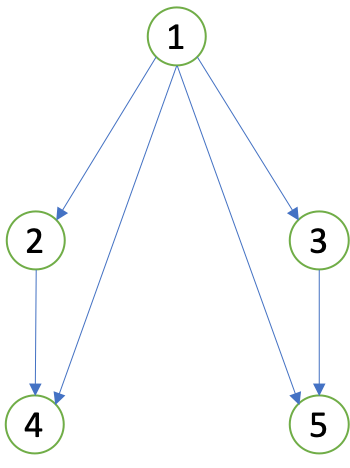
\includegraphics[scale=0.5]{figure/eg1.png}
	\end{center}
\end{figure}
The total ranking is not unique. $\sigma_1=(1,2,3,4,5)$ or $\sigma_2=(1,2,4,3,5)$ both minimize pd loss, but will have different solution in our case. Whether $\sigma_1$ or $\sigma_2$ got outputed depends on $(\mathcal{G}, \mathbf{p})$. If we utilize surrogates from Theorem 6 from \cite{ramaswamy2013convex}, 
\begin{equation*}
\begin{split}
u_2=-y_{12}^{\mathbf{p}}+y_{24}^{\mathbf{p}}\\
u_3 = -y_{13}^{\mathbf{p}}+y_{35}^{\mathbf{p}}\\
u_4 = -y_{24}^{\mathbf{p}}-y_{14}^{\mathbf{p}}\\
u_5 = -y_{35}^{\mathbf{p}}-y_{15}^{\mathbf{p}}\\
\end{split}
\end{equation*}
where according to the graph, $y_{21}^{\mathbf{p}}, y_{42}^{\mathbf{p}}, y_{41}^{\mathbf{p}}, y_{31}^{\mathbf{p}}, y_{51}^{\mathbf{p}}, y_{53}^{\mathbf{p}}=0$. It is easily to see that
\begin{equation*}
\begin{split}
\{y_{12}=100, y_{24}^{\mathbf{p}}=100, y_{13}^{\mathbf{p}}=100, y_{35}^{\mathbf{p}}=99, y_{14}^{\mathbf{p}}=200, y_{15}^{\mathbf{p}}=300\}\Rightarrow \sigma_1\\
\{y_{12}=100, y_{24}^{\mathbf{p}}=100, y_{13}^{\mathbf{p}}=400, y_{35}^{\mathbf{p}}=99, y_{14}^{\mathbf{p}}=200, y_{15}^{\mathbf{p}}=499\}\Rightarrow \sigma_2
\end{split}
\end{equation*}

Although $\sigma_1, \sigma_2$ are equivalent w.r.t pdloss, it is not for our case. Let $c_1=0, c_2=c_3=c_4=c_5=1$. Then if we start from $\sigma_1$, the best $m_1=(1,\{2,3\}, \{4,5\})$ and from $\sigma_2$, the best $m_2=(1,2,\{3,4\}, 5)$. However $m_1$ have smaller target loss. 

To solve this issue, we must go through all possible total ordering. That is, if we have all topological sorting of difference graph, we can run Algorithm 1 on each of them to find out the lowest target loss. Thanks to Theorem 7 of \cite{ramaswamy2013convex}, we will have a calibrated surrogates which will also give us all possible total ordering.

\begin{algorithm}[H]
	\caption{Improved algorithm}
	\begin{algorithmic}[1]
		\Procedure{xxx }{$\mathcal{G}, \mathbf{p}, \mathbf{c}$}
		\State Get $\mathcal{M}$ from Algorithm $1$ from \cite{ramaswamy2013convex}
		\State Let $m^*=NULL$, $loss = \infty$
		\For{\texttt{$\sigma\in\mathcal{M}$}}
		\State
		Let $m=${Clustering ranking }{($\mathcal{G}, \mathbf{p}, \mathbf{c}, \sigma$)}, with $l$ be the corresponding loss.
		\If{\texttt{$l\leq loss$}}
		Set $m^*=m$
		\EndIf
		\EndFor
		\State \textbf{return} $m^*$
		\EndProcedure
	\end{algorithmic}
\end{algorithm}

Warning: this algorithm only works under the assumption that $\mathcal{M}$ is small. If $\mathcal{M}$ is huge, then it would be hard to solve the problem quickly. Consider a DAG over $r$ items($r$ is even), with edges $\{(i,i+1)\}_{i=1}^{r/2}\cup \{(i,i+1)\}_{r/2+1}^r$. Then $|\mathcal{M}|=(\frac{r}{2}+1)!$. 

\end{comment}









\section{Online Learning with Hierarchical Experts}\label{sec:online}
In this section we look at an online decision making problem with structured/dependent experts. In online decision making, we have a finite number of experts $N$ and a finite number of rounds $T$. At each round we have to play an expert after which a loss value for each expert is revealed. The goal is to minimize the total loss incurred. There are many algorithms for this problem but the update time at each round depends linearly on $N$. In cases where the experts are structured (such as paths in a graph), under some structural assumptions on the losses, we can get much faster algorithms such as the ones presented in \cite{koolen2010hedging} and \cite{cortes2015line}. 

Motivated by hierachical classification studied in \cite{ramaswamy2015convex}, we look at experts arranged in a hierachical structure. For example, suppose every day one has to send one person from the Science school to attend a quiz. The exact topic of the quiz is unknown except for the fact that it will be a sub-field of Science. The experts are people with expertice in different branches of Science. Some have a broad knowledge of general topics such as Chemistry or Physics while some might have knowledge about very specific topics such as String Theory or Electrochemistry. In such cases the experts are naturally arranged in a tree. We formalize this as an online decision making problem with structure and provide a solution based on \cite{cortes2015line}.

\subsection{The Problem}
We have a complete rooted binary tree $\Tr$ of height $n$ with each node representing an expert. Given two nodes $y_1$ and $y_2$, let $d_\Tr(y_1,y_2)$ denote the tree distance between the two nodes, i.e., the length of the unique path from $y_1$ to $y_2$ in $\Tr$. The learning proceeds in rounds of interaction between the learner $\L$ and the environment as follows:\\

Learner $\L$: For $t = 1,...,T$,
\begin{itemize}
 \item Play expert $\hat{y}_t \in V(\Tr)$
 \item Receive best expert $y_t \in V(\Tr)$
 \item Incur loss $d_\Tr(\hat{y}_t,y_t)$
 \item Update model
\end{itemize}
We allow the learner to randomize the choice of $\hat{y}_t$ but the environment's choice of $y_t$ only depends on the probability distribution of $\hat{y}_t$ and not on the actual expert played. If we look at the quiz example, we can assume we have one expert for every topic and the true label gives the topic of the quiz on the particular day. Note that the tree need not be binary, but we assume binary trees for the sake of simplicity. 

Since there are only $N = 2^{n+1} - 1$ experts, we can associate a unique number to every expert in the range $[2^{n+1}-1]$ and hence each expert can be represented using only $O(n)$ bits. A more natural representation of each expert is using the location with respect to the root. The vertices of the binary tree $\Tr$ is taken to be $\{w \in \{0,1\}^* \mid |w| \leq n\}$ which is the set of binary sequences of length atmost $n$ and the parent of a node $w$ is obtained by removing the last bit from $w$. The root is repesented by the empty string $\epsilon$, $0$ is a child of $\epsilon$, $01$ is a child of $0$ and so on. The two representations are polynomial time inter-convertible as long as the numbering in the former representation is done in some natural way. We'll use the string/word based representation throughout the rest of this discussion.

The goal of a learning algorithm is twofold: (a) Play step and Update step runs in time polynomial in $n$ and does not depend on $N$. (b) For all sequences of true experts $y_1,...,y_T$, the regret is sub-linear in $T$, where the regret of a learner $\L$ is the total loss incurred minus the loss of the best expert in hindsight:
$$R(\L) = \sum_{t=1}^T d_\Tr(\hat{y}_t,y_t) - \min_{y \in V(\Tr)}\sum_{t=1}^T d_{\Tr}(y,y_t)$$

\textit{Non-linearity of the loss}: Note that the loss $d_\Tr$ is not linear in its first component with the string based representation of nodes. Nonetheless, can we represent each node $y$ as a vector $\u_y$ in $\{0,1\}^d$ and assign a loss vector $\lb_y \in \R_+^d$ to every node such that $d_\Tr(y_1,y_2) = \u_{y_1}^T\lb_{y_2}$? If we could, for small $d$, then we can apply the Component Hedge algorithm from \cite{koolen2010hedging}. But note that $d$ has to be atleast the rank of the $N$-by-$N$ matrix $M_\Tr$ given by $M_\Tr[y_1,y_2] = d_\Tr(y_1,y_2)$. We expect the rank of $M_\Tr$ to be high, although we are not aware of any known bounds.

\subsection{Background}
Our algorithm reduces this problem to the problem studied in Cortes et. al. 2015 \cite{cortes2015line} in which the authors study a class of problems in the online prediction with expert advice setting. In this setting, there is a prediction space $\Y$ and a finite number of experts. There is loss function $\ell:\Y\times\Y \to \R$. At each round $t$, a prediction/advice (in $\Y$) from each expert is revealed using which the learner predicts a $\hat{y}_t \in \Y$. Then the ``correct'' prediction $y_t$ is revealed and the learner incurs loss $\ell(\hat{y_t},y_t)$. 

To state the exact problem studied in the paper, we need some definitions. Let $\Sigma$ be a finite aphabet. Here, we set $\Sigma = \{0,1\}$. A finite automaton $A$ over $\Sigma$ is a tuple $(\Sigma,Q,I,F,E)$ where $Q$ is a finite set of states, $I\subseteq Q$ is the set of initial states, $F\subseteq Q$ is the set of final states and $E \subseteq Q \times (\Sigma \cup \epsilon) \times Q$ is a finite set of transitions (labeled edges) from state to state. We take the prediction space $\Y = \Sigma^*$. Every path from a state in $I$ to a state in $F$ is considered as an expert. At each round $t$, new labels on the edges are revealed. The advice of an expert $\xi$ at time $t$, denoted using $\xi(t)$, is the label of the path $\xi$ at time $t$.

The loss function $\ell: \Sigma^* \times \Sigma^* \to \R$ is given by a weighted finite state transducer WFST $\U$ over $\Sigma$. A WFST $\U$ is a tuple $(\Sigma,Q,I,F,E)$ where $Q$ is a finite set of states, $I \subseteq Q$ is the set of initial states, $F \subseteq Q$ is the set of final states and $E \subseteq Q \times (\Sigma\cup\epsilon)^2 \times \R_+ \times Q$ is a finite set of edges labeled by an input symbol, an output symbol and a weight. For any two strings $y_1,y_2 \in \Sigma^*$, let $P_\U(y_1,y_2)$ denote the set of paths from a state in $I$ to a state in $F$ with the input and output labels of the path being $y_1$ and $y_2$ respectively. The value of an input-output pair $(y_1,y_2) \in \Sigma^*\times\Sigma^*$ denoted by $\U(y_1,y_2)$ is the sum over all paths in $P_\U(y_1,y_2)$ the product of edge weights on the path.
$$\U(y_1,y_2) = \sum_{\pi \in P_\U(y_1,y_2)}\prod_{e\in\pi}\text{weight}(e)$$
where $\text{weight}((q_1,a_i,a_o,r,q_2)) = r$ and a path $\pi$ is viewed as a multiset of edges from $E$. $\U(y_1,y_2)$ is defined to be $0$ if $P_\U(y_1,y_2) = \emptyset$. The corresponding loss function $\ell_\U:\Sigma^*\times\Sigma^* \to \R$ is given by,
$$\ell_\U(y_1,y_2) = -\log(\U(y_1,y_2))$$
Finally, the online learning setting is as follows: There is a WFST $\U$ and a finite automaton $A$ whose (fixed) set of paths is the set of experts.

For rounds $t = 1,...,T$,
\begin{itemize}
 \item Receive new labels on edges of $A$
 \item Play $\hat{y}_t \in \Sigma^*$ based on predictions $\xi(t)$ of each expert $\xi$
 \item Receive correct prediction $y_t \in \Sigma^*$
 \item Incur loss $\ell_\U(\hat{y}_t,y_t)$
 \item Update model
\end{itemize}

The paper provides a Follow The Perturbed Leader (FTPL) based algorithm for this problem that runs in time polynomial in the size of $A$, $\U$ and $T$ if the underlying graphs are acyclic. The regret is also bounded by a constant.

\subsection{Reduction}

We can easily cast our hierarchical experts problem in the above language. Consider the following finite automaton $A$:
\begin{center}
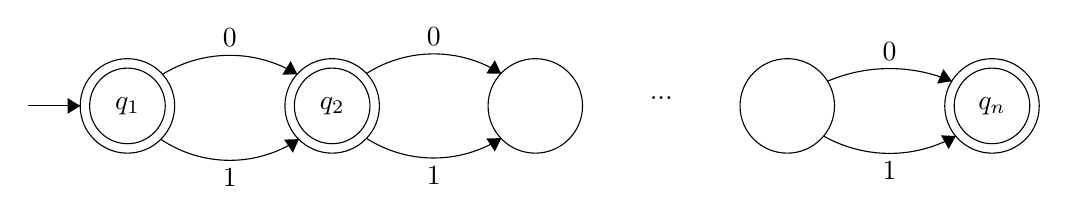
\begin{tikzpicture}[scale=0.2]
\tikzstyle{every node}+=[inner sep=0pt]
\draw [black] (8.8,-27.7) circle (3);
\draw (8.8,-27.7) node {$q_1$};
\draw [black] (8.8,-27.7) circle (2.4);
\draw [black] (21.8,-27.7) circle (3);
\draw (21.8,-27.7) node {$q_2$};
\draw [black] (21.8,-27.7) circle (2.4);
\draw [black] (34.7,-27.7) circle (3);
\draw [black] (50.7,-27.7) circle (3);
\draw [black] (63.7,-27.7) circle (3);
\draw (63.7,-27.7) node {$q_n$};
\draw [black] (63.7,-27.7) circle (2.4);
\draw [black] (11.013,-25.7) arc (121.60326:58.39674:8.18);
\fill [black] (19.59,-25.7) -- (19.17,-24.85) -- (18.64,-25.71);
\draw (15.3,-23.99) node [above] {$0$};
\draw [black] (19.693,-29.81) arc (-55.91527:-124.08473:7.839);
\fill [black] (19.69,-29.81) -- (18.75,-29.84) -- (19.31,-30.67);
\draw (15.3,-31.66) node [below] {$1$};
\draw [black] (23.966,-25.65) arc (122.61963:57.38037:7.948);
\fill [black] (32.53,-25.65) -- (32.13,-24.8) -- (31.59,-25.64);
\draw (28.25,-23.9) node [above] {$0$};
\draw [black] (32.536,-29.752) arc (-57.3416:-122.6584:7.943);
\fill [black] (32.54,-29.75) -- (31.59,-29.76) -- (32.13,-30.6);
\draw (28.25,-31.51) node [below] {$1$};
% \draw [black] (37.7,-27.7) -- (47.7,-27.7);
% \fill [black] (47.7,-27.7) -- (46.9,-27.2) -- (46.9,-28.2);
\draw (42.7,-27.2) node  {$...$};
\draw [black] (53.246,-26.135) arc (113.06476:66.93524:10.092);
\fill [black] (61.15,-26.13) -- (60.61,-25.36) -- (60.22,-26.28);
\draw (57.2,-24.83) node [above] {$0$};
\draw [black] (61.404,-29.606) arc (-60.40346:-119.59654:8.511);
\fill [black] (61.4,-29.61) -- (60.46,-29.57) -- (60.95,-30.44);
\draw (57.2,-31.22) node [below] {$1$};
\draw [black] (2.5,-27.7) -- (5.8,-27.7);
\fill [black] (5.8,-27.7) -- (5,-27.2) -- (5,-28.2);
\end{tikzpicture}
\end{center}
There are $n$ linearly arranged states with two transitions from one state to the next (one for each label 0 and 1). $q_1$ is the only initial state and every state is a final state. Hence, every path uniquely represents a node in the tree $\Tr$, specifically, the node represented by the label on the path. In our case, the advice of each expert/path remains the same for each round and is exacly the representation of the expert/node in $\Tr$. Now we need to represent the loss $d_{\Tr}$ using a WFST $\U$. Such a $\U$ is given below. The input and output labels on the edges are separated by a `$/$' and the weight is given in paranthesis.

\begin{center}
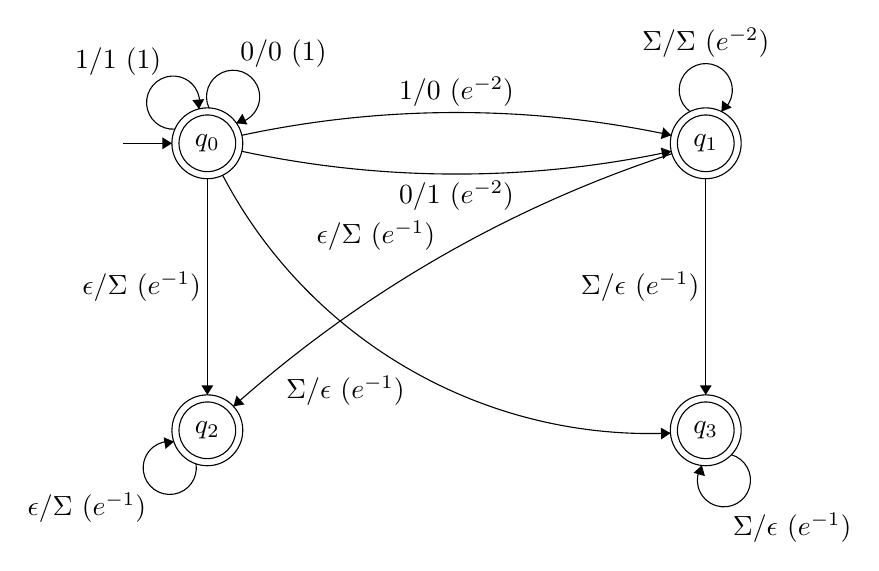
\begin{tikzpicture}[scale=0.15]
\tikzstyle{every node}+=[inner sep=0pt]
\draw [black] (19.8,-13.6) circle (3);
\draw (19.8,-13.6) node {$q_0$};
\draw [black] (19.8,-13.6) circle (2.4);
\draw [black] (62,-13.6) circle (3);
\draw (62,-13.6) node {$q_1$};
\draw [black] (62,-13.6) circle (2.4);
\draw [black] (19.8,-37.9) circle (3);
\draw (19.8,-37.9) node {$q_2$};
\draw [black] (19.8,-37.9) circle (2.4);
\draw [black] (62,-37.9) circle (3);
\draw (62,-37.9) node {$q_3$};
\draw [black] (62,-37.9) circle (2.4);
\draw [black] (12.7,-13.6) -- (16.8,-13.6);
\fill [black] (16.8,-13.6) -- (16,-13.1) -- (16,-14.1);
\draw [black] (19.941,-10.615) arc (205.03398:-82.96602:2.25);
\draw (26.25,-7.19) node [above] {$0/0\mbox{ }(1)$};
\fill [black] (22.25,-11.9) -- (23.19,-12.01) -- (22.77,-11.1);
\draw [black] (17.063,-12.4) arc (274.05479:-13.94521:2.25);
\draw (12.25,-7.94) node [above] {$1/1\mbox{ }(1)$};
\fill [black] (19.09,-10.7) -- (19.53,-9.86) -- (18.53,-9.94);
\draw [black] (22.722,-12.92) arc (102.10355:77.89645:86.695);
\fill [black] (59.08,-12.92) -- (58.4,-12.26) -- (58.19,-13.24);
\draw (40.9,-10.49) node [above] {$1/0\mbox{ }(e^{-2})$};
\draw [black] (59.078,-14.279) arc (-77.90311:-102.09689:86.742);
\fill [black] (59.08,-14.28) -- (58.19,-13.96) -- (58.4,-14.94);
\draw (40.9,-16.71) node [below] {$0/1\mbox{ }(e^{-2})$};
\draw [black] (60.677,-10.92) arc (234:-54:2.25);
\draw (62,-6.35) node [above] {$\Sigma/\Sigma\mbox{ }(e^{-2})$};
\fill [black] (63.32,-10.92) -- (64.2,-10.57) -- (63.39,-9.98);
\draw [black] (19.8,-16.6) -- (19.8,-34.9);
\fill [black] (19.8,-34.9) -- (20.3,-34.1) -- (19.3,-34.1);
\draw (19.3,-25.75) node [left] {$\epsilon/\Sigma\mbox{ }(e^{-1})$};
\draw [black] (22.008,-35.869) arc (131.79304:108.07616:104.244);
\fill [black] (22.01,-35.87) -- (22.94,-35.71) -- (22.27,-34.96);
\draw (34.07,-22.74) node [above] {$\epsilon/\Sigma\mbox{ }(e^{-1})$};
\draw [black] (18.84,-40.73) arc (9:-279:2.25);
\draw (9.6,-43.15) node [below] {$\epsilon/\Sigma\mbox{ }(e^{-1})$};
\fill [black] (16.97,-38.86) -- (16.1,-38.49) -- (16.26,-39.48);
\draw [black] (62,-16.6) -- (62,-34.9);
\fill [black] (62,-34.9) -- (62.5,-34.1) -- (61.5,-34.1);
\draw (61.5,-25.75) node [left] {$\Sigma/\epsilon\mbox{ }(e^{-1})$};
\draw [black] (59.01,-38.138) arc (-87.55222:-152.31699:40.846);
\fill [black] (59.01,-38.14) -- (58.19,-37.67) -- (58.23,-38.67);
\draw (31.49,-33.23) node [below] {$\Sigma/\epsilon\mbox{ }(e^{-1})$};
\draw [black] (64.159,-39.966) arc (73.98311:-214.01689:2.25);
\draw (69.31,-44.89) node [below] {$\Sigma/\epsilon\mbox{ }(e^{-1})$};
\fill [black] (61.67,-40.87) -- (60.97,-41.5) -- (61.93,-41.78);
\end{tikzpicture}
\end{center}

$q_0$ is the only initial state and every state is a final state. The underlying automaton of $\U$  automaton is determiistic and $P_\U(y_1,y_2)$ is a singleton for every pair of experts $y_1$ and $y_2$. The transducer ignores the longest common prefix and multiplies $e^{-2}$ as long as both strings still have symbols to be read and then multiplies $e^{-1}$ for the rest of the remaining string. It is easy to see that for any two experts/nodes in $\Tr$, $y_1$ and $y_2$, $\U(y_1,y_2) = \exp(-d_{\Tr}(y_1,y_2))$ giving us that $\ell_{\U}(y_1,y_2) = d_{\Tr}(y_1,y_2)$. Note that $\U$ is not acyclic but can be made acyclic by making $n$ copies and adding transitions from one copy to another.

Hence if we use the solution from \cite{cortes2015line} with the automaton $A$ (same label for every time step) and loss given by $\U$, we get a solution running in time polynomial in $|A|$, $|\U|$ and $T$ and hence polynomial in $n$ and $T$. The regret bound we get is,
$$\E[R(\L)] \leq 8n\sqrt{N(1+2\log(n))L_{min}} + 64n^2N(1+2\log(n))$$
The expectation is under the randomness of the algorithm and $L_{min}$ is the cumulative loss of the best expert in hindsight. 

\subsection{Further Work}
Although the runtime is polynomial in $n$ and does not depend on $N$, the solution uses an FTPL style algorithm causing the memory used and time taken in round $t$ to be linear in $t$ which is not feasible in most cases. Also, the regret bound, inspite of being sublinear in $T$, depends on $N$ which is large. One possible direction is to design a new online learning algorithm directly for the hierarchical experts case that does not have such limitations.

\newpage
%============================= BIBLIOGRAPHY ===============================

\bibliographystyle{plain}
\bibliography{biblio}


\end{document}

%=========================== END DOCUMENT ==============================
